
% Lecture 09 - 2024-01-29
\section{Cylindrical coordinates}
\begin{itemize}
    \item Cylindrical coordinates represent a point $P(x,y,z)$ in space by ordered triples $(r,\theta, z)$ in which $(r,\theta)$ is the polar coordinate of $(x,y)$.
    \item $z$ remains unchanged.
    \begin{equation*}
    \fbox{$
    \qquad
        \begin{cases}
            \begin{aligned}
                x &= r\cos \theta \\
                y &= r\sin \theta \\
                z &= z 
            \end{aligned}
        \end{cases} \qquad 
        \text{and}\qquad 
        \begin{cases}
            \begin{aligned}
                r^2 &= x^2 + y^2  \\
                \frac{y}{x} &= \tan \theta .
            \end{aligned}
        \end{cases}
        \qquad
        $}
    \end{equation*}
    \begin{center}
        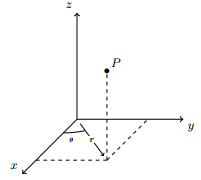
\includegraphics[scale=0.7]{images/09-cylindrical.png}
    \end{center}
    \item \underline{\textbf{Example.}} Change $(x,y,z) = (-1,1,1)$ into cylindrical coordinates.
    \begin{proof} $r^2 = x^2+y^2 = 2$, thus $r=\sqrt{2}$. Then $\tan\theta = \frac{y}{x} = \frac{1}{-1} = -1$, thus $\theta = \frac{3\pi}{4}$. Hence 
    $$(-1,1,1)\mapsto \left(\sqrt{2}, \frac{3\pi}{4}, 1\right).$$
    \end{proof}
    \item \underline{\textbf{Example.}} Change $(\sqrt{2}, 3\pi/4, 2)$ to Cartesian coordinates.
    \begin{proof} We have $x = r\cos \theta = \sqrt{2}\times \left(-\frac{1}{\sqrt{2}}\right) = -1$ and $y = r\sin \theta = \sqrt{2}\times \left(\frac{1}{\sqrt{2}}\right) = 1$. Thus 
    $$(\sqrt{2}, 3\pi/4, 2)\mapsto (1,-1, 2).$$
    \end{proof}
\end{itemize}

\section{Spherical coordinates}
\begin{itemize}
    \item $(x,y,z)\mapsto (\rho, \theta,\phi)$, where basically we repeat the polar coordinate first, and the \emph{height} $z$ is tracked via the variable $\phi$, the angle with $Oz$. 
    Note that the order is sometime written as $(r,\phi, \theta)$. \textbf{Pay attention to the order!}
    \item The relations, still introducing an extra variable $r$ as in polar coordinates (it will be very useful)\color{red}
    \begin{equation*}
    \fbox{$
    \qquad
        \begin{cases}
            \begin{aligned}
                x &= (\rho \sin \phi) \cos \theta \\
                y &= (\rho \sin \phi) \sin \theta \\
                z &= \rho \cos \phi
            \end{aligned}
        \end{cases} \qquad 
        \text{and}\qquad 
        \begin{cases}
            \begin{aligned}
                 \rho^2 &= x^2+y^2+z^2 \\
                r &= \rho \sin \phi \\
                \frac{r}{z} &= \tan \phi
            \end{aligned}
        \end{cases}, \qquad \theta \in  [0,2\pi], \phi\in [0,\pi]
        \qquad
        $}
    \end{equation*}
    \begin{center}
        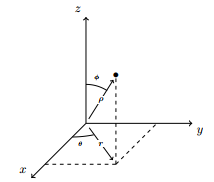
\includegraphics[scale=0.7]{images/09-spherical.png}
    \end{center}\color{black}
    \item If $\phi > \frac{\pi}{2}$ then $z<0$, the angle make $P$ lies below the $Oxy$-plane.
    
    \item \underline{\textbf{Example.}} Convert $(1,1,0)$ into spherical coordinate.
    \begin{proof} $\rho^2 = x^2+y^2+z^2 = 2$, thus $\rho = \sqrt{2}$. Now $z = \rho \cos \phi$ implies $0 = \sqrt{2} \cos \phi$, thus $\phi = \frac{\pi}{2}$. Finally $\tan\theta = \frac{y}{x} = 1$, thus $\theta = \frac{\pi}{4}$ (since $x>0, y>0$). We conclude 
    \begin{equation*}
        (1,1,0) \mapsto \left(\sqrt{2}, \frac{\pi}{4}, \frac{\pi}{2}\right) = (r,\theta, \phi).
    \end{equation*}
    \end{proof}

    \item \underline{\textbf{Example.}}  True/False: Consider the point with spherical coordinates $(\rho, \theta,\phi)=(4, \frac{3\pi}{4}, \frac{5\pi}{7})$. The product of the Cartesian coordinates, $xyz$, is positive.
    \begin{proof} \textbf{True}. We see that $\phi = \frac{5\pi}{7} > \frac{\pi}{2}$, thus $z<0$. Now $\theta = \frac{3\pi}{4}$, thus $x>0, y<0$ (draw a picture). Therefore $xyz>0$.
    \end{proof}
\end{itemize}
\section{Practice}
\begin{itemize}

    \item \underline{\textbf{Example.}} Convert the equation $z = \sqrt{x^2+y^2}$ into cylindrical coordinates and spherical coordinates.
    \begin{proof}\quad 
        \begin{itemize}
            \item Cylindrical: $z = r$.
            \item Spherical: $\rho \cos \phi = r = \rho \sin \phi$, thus $\tan \phi = 1$, thus $\phi = \frac{\pi}{4}$ is the equation of the cone!
        \end{itemize}
    \end{proof}
    
    \item \underline{\textbf{Example.}} Identify the surface whose equation is $z = 4-r^2$ in cylindrical coordinate.
    \begin{proof}
        We have $z = 4 - x^2-y^2$, thus this is a elliptical paraboloid (one term of 1st order, two terms of second order having the same sign).
    \end{proof}

    \item \underline{\textbf{Example.}} Convert to $x,y,z$ the surface: $\rho = \sin \phi\cos \phi$.
    \begin{proof} We can do 
    \begin{equation*}
        (x^2+y^2+z^2)^\frac{3}{2}= \rho^3 = (\rho \sin \phi) (\rho\cos \phi) = rz = z\sqrt{x^2+y^2}.
    \end{equation*}
    The answer is $(x^2+y^2+z^2)^\frac{3}{2} = z\sqrt{x^2+y^2}$.
    \end{proof}

    \item \underline{\textbf{Example.}} Identify the surface whose equation is: $\rho = \sin \phi\cos \theta$.
    \begin{proof} We can do 
    \begin{equation*}
        x^2+y^2+z^2 =\rho^2 = (\rho \sin \phi) \cos \theta = r\cos\theta = x
    \end{equation*}
    Therefore 
    \begin{equation*}
        \left(x-\frac{1}{2}\right)^2 + y^2 +z^2 = \frac{1}{4}
    \end{equation*}
    This is a sphere centered at $(\frac{1}{2},0,0)$ with radius $\frac{1}{2}$, this is a \emph{ellipsoid}.
    \end{proof}
\end{itemize}